\begin{pastexam}[label={px:nsysu-108-osds-02}]{中山資工所甲組 108 學年度 第 2 題}
（問答、追蹤）

\textbf{[Advanced Data Structures: 20\%]}
\begin{enumerate}[label=(\arabic*)]
\item Given a directed graph G = (V, E), what is its strongly connected component? (4\%)
\item Using a B-tree to maintain disk blocks helps reduce the cost of disk access. Why? (4\%)
\item What is the difference between a B$^+$-tree and a B$^*$-tree? (4\%)
\item What are the two properties of a binomial-heap? (4\%)
\item Consider a Fibonacci heap as follows:
\begin{center}
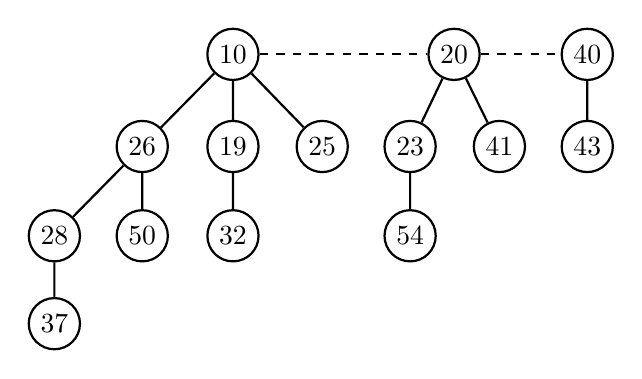
\begin{tikzpicture}[x=0.9cm,y=0.9cm,
  n/.style={circle,draw,thick,inner sep=0pt,minimum size=6.5mm},every path/.style={thick}]
  \node[n] (10) at (2.52,0) {10}; \node[n] (20) at (5.64,0) {20}; \node[n] (40) at (7.52,0) {40};
  \node[n] (26) at (1.24,-1.3) {26}; \node[n] (19) at (2.52,-1.3) {19}; \node[n] (25) at (3.78,-1.3) {25};
  \node[n] (23) at (5.02,-1.3) {23}; \node[n] (41) at (6.28,-1.3) {41}; \node[n] (43) at (7.52,-1.3) {43};
  \node[n] (28) at (0,-2.56) {28}; \node[n] (50) at (1.24,-2.56) {50}; \node[n] (32) at (2.52,-2.56) {32};
  \node[n] (54) at (5.02,-2.56) {54};
  \node[n] (37) at (0,-3.8) {37};
  \draw[dashed] (10)--(20)--(40);
  \draw (10)--(26) (10)--(19) (10)--(25) (26)--(28) (26)--(50) (28)--(37) (19)--(32)
        (20)--(23) (20)--(41) (23)--(54) (40)--(43);
\end{tikzpicture}
\end{center}
The number in each node gives its key value. Suppose that we decrease key 50 to 18 and then
decrease key 37 to 7. Show the result of the revised heap. (4\%)
\end{enumerate}
\end{pastexam}

\begin{pastsoln}
五個小題分屬不同章：(1) 強連通元件（資結書第~23.1~節）、(2)(3) B 樹與 B$^{+}$ 樹（第~11.2、11.3~節）、
(4)(5) 二項堆積與費氏堆積（第~8.5、8.6~節）。 本書把整題放在第~8~章。

\textbf{(1)} 有向圖 $G = (V, E)$ 的強連通元件（strongly connected component, SCC）是一個\textbf{極大}的頂點
集合 $C \subseteq V$，其中任兩個頂點 $u, v$ 互相可達：有 $u$ 到 $v$ 的路徑，也有 $v$ 到 $u$ 的路徑
（資結書第~23.1~節）。 「互相可達」是等價關係，SCC 就是它的等價類，所以每個頂點恰好屬於一個 SCC。 把
每個 SCC 縮成一點得到的分量圖一定是 DAG。 求法：Kosaraju 或 Tarjan，都是 $O(|V| + |E|)$。

\textbf{(2)} 磁碟以區塊為單位讀寫，讀一個區塊比在記憶體裡比較幾百次還慢得多，所以磁碟上的資料結構，成本
幾乎只看讀了幾個區塊（資結書第~11.3.1~節）。 B 樹讓一個節點剛好占一個區塊，一個節點裡放幾十到幾百個
鍵，分支度很大，樹高只有 $O(\log_t n)$（資結書定理~11.1）。 查一筆資料只要從根走到葉，讀的區塊數就是
樹高，例如 $10^8$ 筆資料大約 $3$ 到 $4$ 個區塊；同樣的資料放在二元搜尋樹裡，高度至少 $\lg 10^8 \approx 27$，
每往下一層都可能讀一個不同的區塊。 另外 B 樹每個節點至少半滿，空間使用率有保證，插入刪除也只動到一條
路徑上的 $O(\log_t n)$ 個區塊。

\textbf{(3)} 兩者都是 B 樹的變形，改的地方不同：
\begin{itemize}
\item \textbf{B$^{+}$ 樹}改的是\textbf{資料放在哪裡}：所有鍵和資料（或記錄指標）都在葉子，內部節點只放
分隔鍵（葉子某些鍵的複本），葉子由左到右串成串列（資結書第~11.3~節）。 好處是內部節點放得下更多
分隔鍵、樹更矮，而且範圍查詢、依序走訪只要沿葉子串列走。
\item \textbf{B$^*$ 樹}改的是\textbf{節點多滿、怎麼分裂}：根以外的節點至少三分之二滿；節點滿了先把鍵轉給
相鄰的兄弟，兄弟也滿了才把兩個滿的節點分成三個（2 分 3）。 好處是空間使用率較高、分裂較少。
\end{itemize}
一句話：B$^{+}$ 樹把資料全部移到串起來的葉子；B$^*$ 樹提高每個節點的最低填滿率。 （B$^*$ 樹不在資結書裡。）

\textbf{(4)} 二項堆積是一群二項樹，滿足（資結書第~8.5~節）：
\begin{enumerate}[label=(\roman*)]
\item 每一棵二項樹都滿足（最小）堆積性質：每個節點的鍵不小於父節點的鍵，所以最小值在某一棵樹的根。
\item 每個階數最多只有一棵二項樹。 因此 $n$ 個元素的二項堆積由哪些樹組成是固定的：$n$ 的二進位第 $k$ 位是
$1$，就有一棵 $B_k$；樹最多 $\lfloor \lg n \rfloor + 1$ 棵。
\end{enumerate}

\textbf{(5)} 費氏堆積的減少鍵值（資結書第~8.6~節）：鍵變小後如果比父節點小，就把它連同子樹剪下來放進
根串列；父節點如果不是根，第一次失去子節點時做標記，已經有標記的再失去子節點就連鎖剪下。 題目的圖沒有
標出任何有標記的節點，下面假設一開始都沒有標記，最小指標指向 $10$。

\textbf{把 50 減為 18}。 $50$ 的父節點是 $26$，$18 < 26$ 違反堆積性質。 剪下 $18$（它沒有子節點），放進
根串列。 $26$ 不是根、原本沒有標記，現在做標記，不再往上。 $18 > 10$，最小指標不變。

\textbf{把 37 減為 7}。 $37$ 的父節點是 $28$，$7 < 28$。 剪下 $7$，放進根串列。 $28$ 不是根、原本沒有標記，
做標記，停止。 $7 < 10$，最小指標改指向 $7$。

結果（灰色是有標記的節點；新剪下的根接在根串列最後，根串列的順序不影響正確性）：
\begin{center}
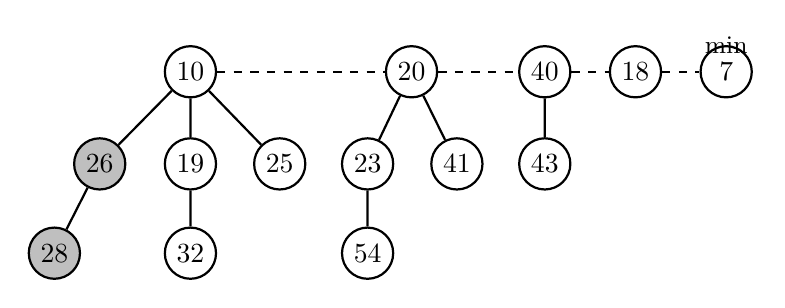
\begin{tikzpicture}[x=0.9cm,y=0.9cm,
  n/.style={circle,draw,thick,inner sep=0pt,minimum size=6.5mm},mk/.style={n,fill=black!25},
  every path/.style={thick}]
  \node[n] (10) at (2.52,0) {10}; \node[n] (20) at (5.64,0) {20}; \node[n] (40) at (7.52,0) {40};
  \node[n] (18) at (8.8,0) {18}; \node[n] (7) at (10.08,0) {7};
  \node[mk] (26) at (1.24,-1.3) {26}; \node[n] (19) at (2.52,-1.3) {19}; \node[n] (25) at (3.78,-1.3) {25};
  \node[n] (23) at (5.02,-1.3) {23}; \node[n] (41) at (6.28,-1.3) {41}; \node[n] (43) at (7.52,-1.3) {43};
  \node[mk] (28) at (0.6,-2.56) {28}; \node[n] (32) at (2.52,-2.56) {32};
  \node[n] (54) at (5.02,-2.56) {54};
  \draw[dashed] (10)--(20)--(40)--(18)--(7);
  \draw (10)--(26) (10)--(19) (10)--(25) (26)--(28) (19)--(32)
        (20)--(23) (20)--(41) (23)--(54) (40)--(43);
  \node[font=\small,above=1mm] at (7) {min};
\end{tikzpicture}
\end{center}
根串列：$10, 20, 40, 18, 7$，最小值是 $7$。 $10$ 的子節點 $26$（有標記）只剩一個子節點 $28$（有標記，
沒有子節點）。 其他樹不變。

如果一開始 $26$ 已經有標記，第一次減少鍵值時 $26$ 也會被剪下（連鎖剪下）成為新的根並清除標記，$10$ 是根
不做標記；考卷沒有標示，就照「都沒有標記」作答，並寫出這個假設。
\end{pastsoln}
